\section{Anwendungsszenario 1: Triviale Navigation}
Das erste Szenario dient auf der einen Seite dem Nachweis der Grundfunktionen der Navigation. Auf der anderen Seite wird das simple Beispiel genutzt, um die Bedienung und Auswertung des Experiment mittels \lstinline{RViz}{} zu erläutern. Den Ausgangspunkt aller Experimente stellt die  Karte des Labors dar, die unter Anderem in der folgenden Abbildung zu sehen ist. Die schwarzen Pixel stellen Hindernisse, die hellgrauen freie Flächen und die restlichen undefinierte Flächen dar.
\begin{figure}[!ht]
\centering
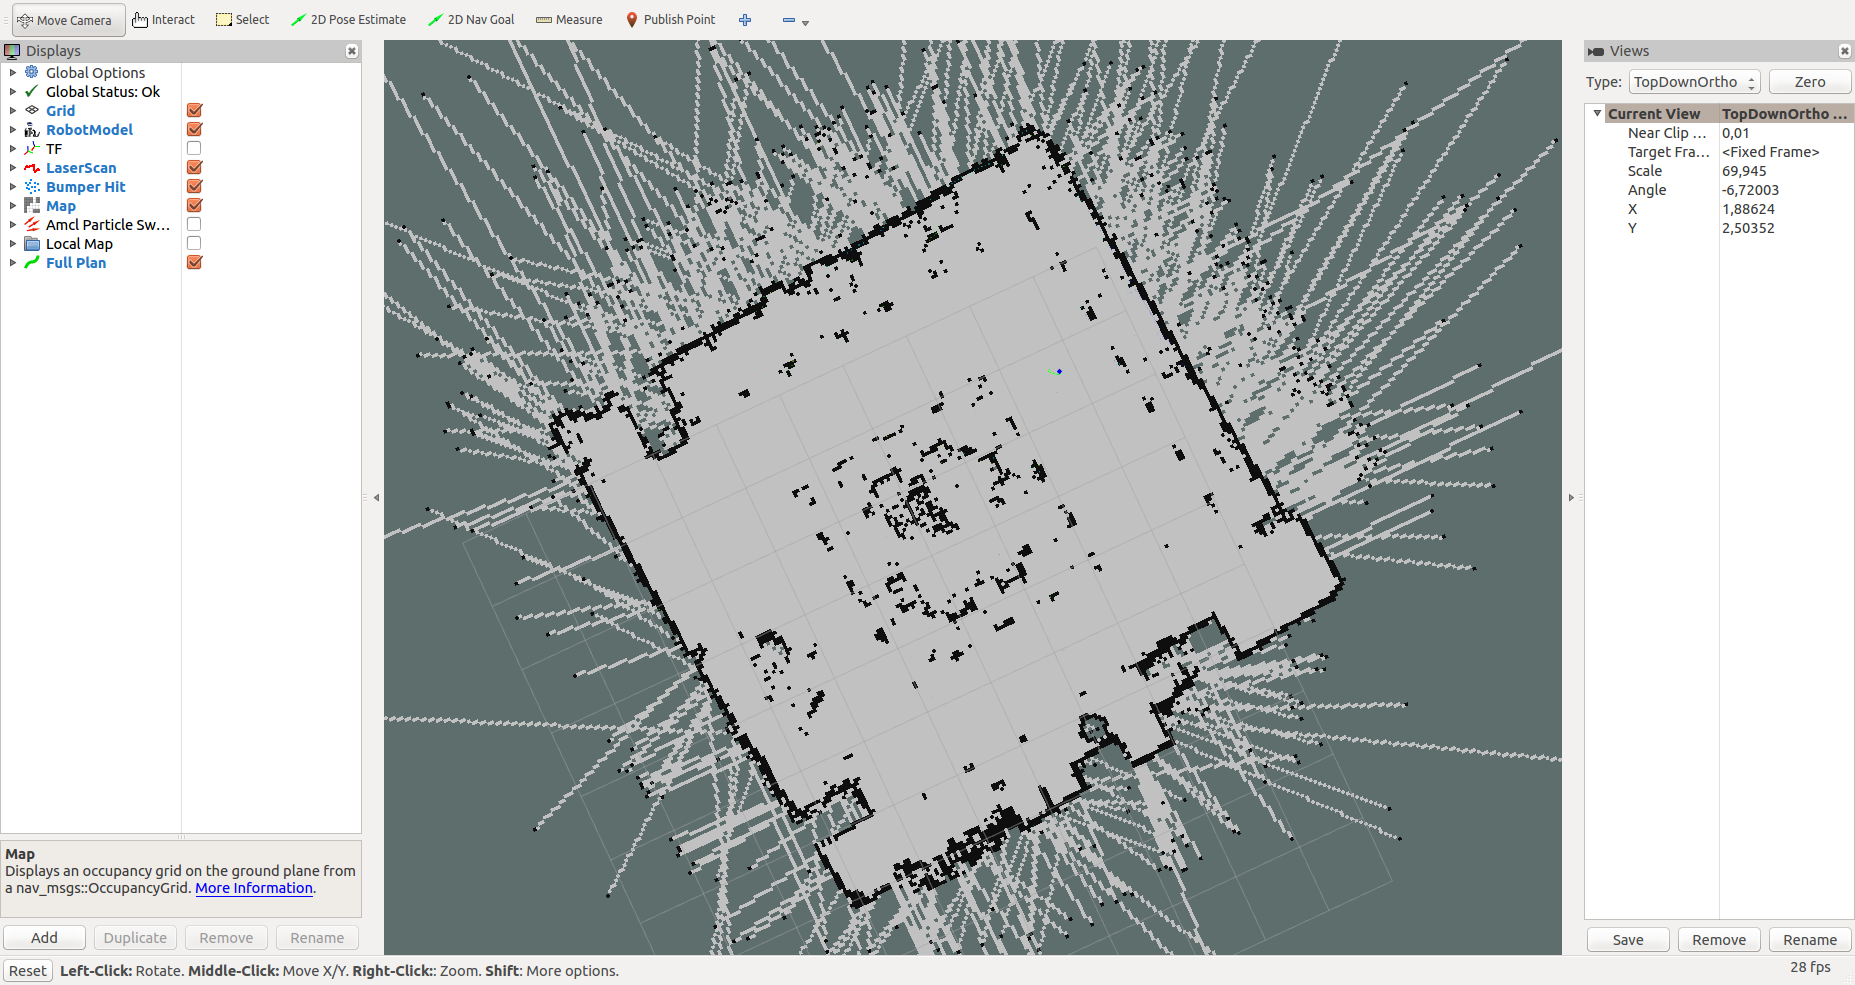
\includegraphics[width=0.8\linewidth]{img/Experiment1_RViz_Overview.png}
\caption{Übersicht von \lstinline{RViz}{}}
\end{figure}
Die Karte wird von \lstinline{RViz}{} angezeigt. Um die Visualisierung zu konfigurieren, können die Elemente auf der linken Seite nach Bedarf an- und abgewählt werden. In der Toolbar können die Elemente \lstinline{2D Pose Estimate}{} und \lstinline{2D Nav Goal}{} genutzt werden, um die eine Positionsschätzung anzugeben und das Ziel der Navigation anzugeben.
Mithilfe Letzteren wird ein Ziel in der entgegengesetzten Ecke des Raums vorgegeben, woraufhin ein globaler Pfad geplant wird, der in der folgenden Abbildung zu sehen ist.
\begin{figure}[!ht]
\centering
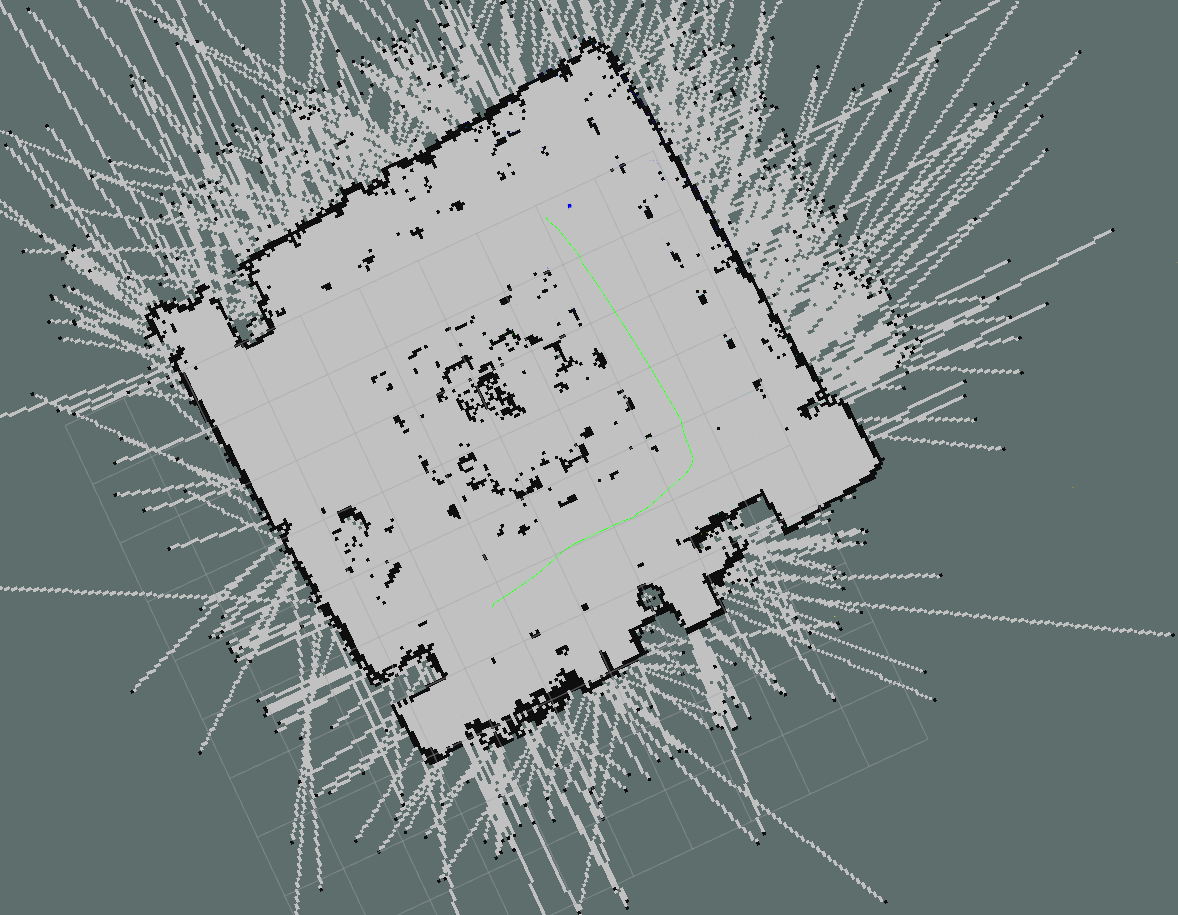
\includegraphics[scale=0.6, trim={7cm 6cm 9cm 3cm},clip]{img/Experiment1_Bild_Fullpath.png}
\caption{Globaler Plan}
\end{figure}

\newpage
Wie der oben eingezeichnete Pfad entsteht, wird recht leicht ersichtlich, wenn die globale Kostenkarte betrachtet wird. Die Bewertung der Zellen beginnt jeweils in den belegten Hindernissen und wird exponentiell fallend von diesen weg propagiert.
\begin{figure}[!ht]
\centering
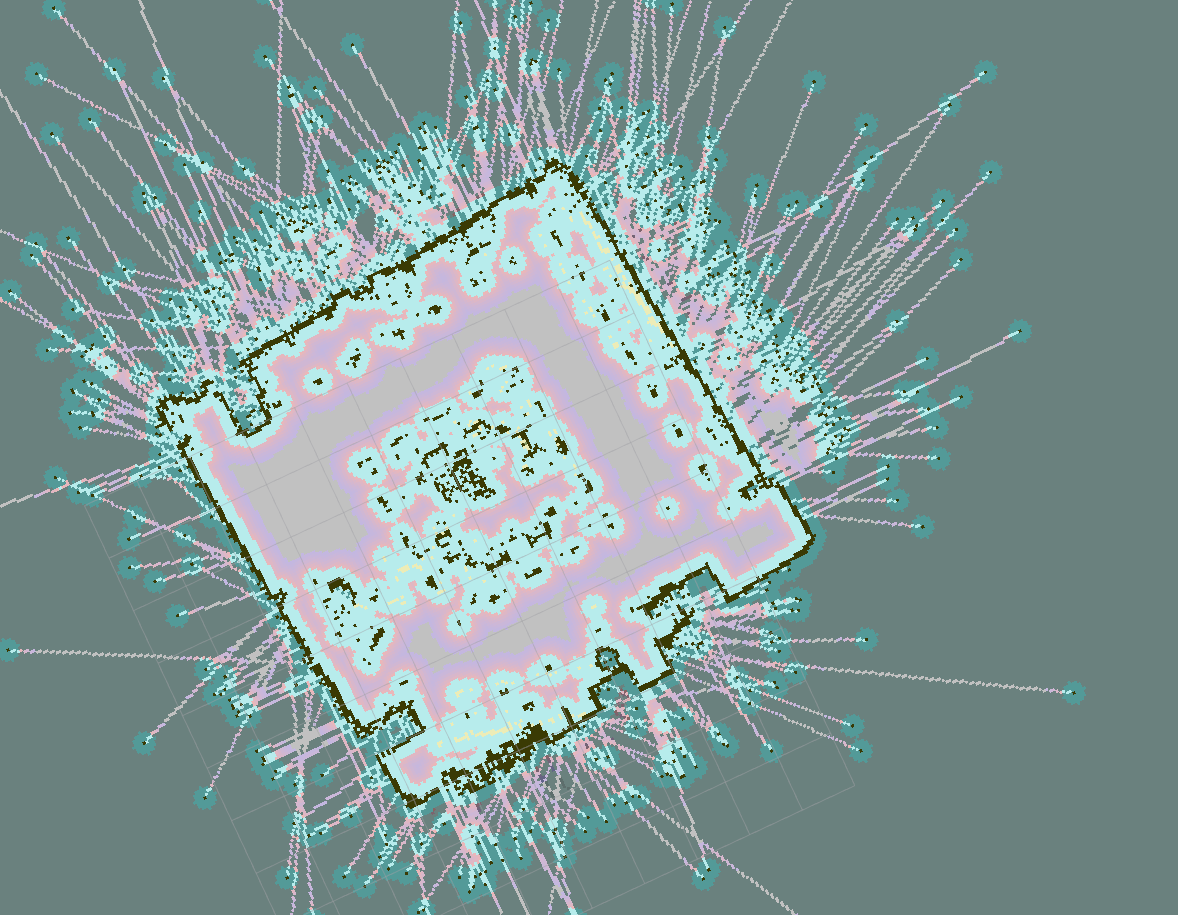
\includegraphics[scale=0.5, trim={4cm 2cm 9cm 3cm},clip]{img/Experiment1_Global_Costmap.png}
\caption{Globale Kostenkarte des Labors}
\end{figure}
Der gezeigt Pfade wurde nach der Planung problemlos von dem Roboter abgefahren, womit die Grundfunktion der Navigation nachgewiesen ist.